\documentclass{article}

\usepackage[utf8]{inputenc}
\usepackage{geometry}
\usepackage{graphicx}

\usepackage{algorithm}% http://ctan.org/pkg/algorithms
\usepackage{algpseudocode}% http://ctan.org/pkg/algorithmicx

\usepackage{hyperref}

\usepackage{float}

\delimitershortfall-1sp
\newcommand\abs[1]{\left|#1\right|}


\title{Algoritmo: Buscar el par de puntos mas cercano en espacio n-dimensional}
\author{Sergio García Prado}


\begin{document}

\begin{titlepage}
	\centering
	{\scshape\LARGE Universidad de Valladolid \par}
	\vspace{1cm}
	{\scshape\Large Algoritmo Divide y vencerás\par}
	\vspace{1.5cm}
	{\huge\bfseries Par de puntos más cercano en espacio n-dimensional\par}
	\vspace{2cm}
	{\Large\itshape Sergio García Prado\par}
	
	\vfill
	Seguimiento del trabajo en: \par
	\href{https://github.com/garciparedes/Closest-Pair-of-Points}{github.com/garciparedes/Closest-Pair-of-Points}

	\vfill


% Bottom of the page
	{\large \today\par}
\end{titlepage}

\section{Introducción}

	\paragraph{}
	El problema que se va a analizar se basa en encontrar el par de puntos más cercanos en un conjunto de puntos pertenecientes a un espacio n-dimensional. Es una condición obligatoria que todos los puntos pertenezca a la misma dimensión ya que de no ser así no tendría sentido comparar sus distancias para encontrar el par mas cercano. Seguidamente se exponen los fundamentos del algoritmo que mejor resuelve el problema.
	
	\subsection{Divide y vencerás}
		
		\paragraph{}
		Divide y Vencerás hace referencia a uno de los paradigmas de diseño de algoritmos mas importantes. Los algoritmos de este tipo por lo general constan de los siguientes pasos:
		
		\paragraph{}
		En primer lugar ha de plantearse el problema de forma que pueda ser descompuesto en k subproblemas del mismo tipo, pero de menor tamaño. Es decir, si el tamaño de la entrada es n, hemos de conseguir dividir el problema en k subproblemas (donde $1 \leq k \leq n$), cada uno con una entrada de tamaño $n/k$ y donde $0 \leq n/k < n$. A esta tarea se le conoce como división.
		
		\paragraph{}
		En segundo lugar han de resolverse independientemente todos los subproblemas, bien directamente si son elementales o bien de forma recursiva. El hecho de que el tamaño de los subproblemas sea estrictamente menor que el tamaño original del problema nos garantiza la convergencia hacia los casos elementales, también denominados casos base.
		
		\paragraph{}
		Por último, combinar las soluciones obtenidas en el paso anterior para construir la solución del problema original.
		
	\subsection{Enfoques para resolver encontrar el par de puntos más cercano}


		\paragraph{}
		Existen distintos enfoques para resolver este problema. El mas simple pero a la vez menos eficiente de todos se basa en comparar todos los puntos con todos e ir guardando los dos que menor distancia tienen entre sí. Esta solución tiene un crecimiento asintótico de $O(n^2)$.

		\paragraph{}
		Tras analizar el problema detenidamente nos damos cuenta de que dados dos puntos A y B, la distancia del punto A al punto B es la misma que del B al A. Por este detalle deducimos que nos podemos ahorrar estas operaciones innecesarias comparando solo una vez los pares entre sí.
	
	
		\paragraph{}
		Profundizando algo mas en nuestro problema vemos que al ser posiciones, estas se pueden subdividir en subconjuntos mas pequeños y así obviar el análisis de pares que estén muy alejados. Este enfoque es del tipo divide y vencerás. En la siguiente sección expondremos con más profundidad las ventajas de esta solución.

		\paragraph{Motivos por los que usar divide y vencerás}

			\begin{enumerate}

				\item
				Los puntos mas cercanos en el espacio por la propia definición de cercanía van a estar en una región próxima del espacio. Este es el motivo por el cual nos podemos ahorrar comparar dos puntos que están muy alejados entre sí en el espacio.
				
				\item
				Si encontramos un mínimo en un subconjunto del espacio y este lo es también para todos los subconjuntos que contienen a este, entonces habremos encontrado el mínimo de todo el espacio.

			\end{enumerate}

\section{Solución implementada (Divide y vencerás)}

	\paragraph{}
	La solución que se ha escogido es la de realizar particiones binarias en el espacio recursivamente hasta tener subconjuntos de pequeño tamaño (En la implementación propuesta como ejemplo se ha fijado en conjuntos de 10 puntos pero teóricamente se debe plantear como conjuntos de 3 elementos, que es el problema de menor tamaño.) para después compararlos utilizando un algoritmo boraz que nos asegura el mínimo local de cada subconjunto. Lo siguiente es quedarse con el mínimo los dos subconjuntos y después analizar los puntos que se encuentran en la frontera que los divide ya que puede darse el caso de que el par de puntos con distancia mínima contuviera el punto 1 perteneciente al primer subconjunto y el punto 2 perteneciente al segundo subconjunto, o viceversa. Si no se evaluase este caso podría darse el caso de que el mínimo encontrado no fuera el real ya que aunque esté en la frontera de los dos subconjuntos pertenece al conjunto que las contiene.
	

	\paragraph{}
	Las explicaciones se van a exponer en un espacio de 3 dimensiones pero estas son extrapolables a cualquier dimensión.

	\subsection{Division}
		
		\paragraph{}
		Lo que intentamos conseguir al dividir el espacio en subconjuntos de forma recursiva es agrupar los puntos que están más próximos, es decir, que la distancia máxima que se pueda encontrar el subconjunto sea la mínima posible para así prescindir del mayor número de comparaciones posibles. 
		
		\paragraph{}
		Vamos a suponer que nuestro conjunto de puntos no está ordenado por lo que lo primero que haremos será ordenarlo sobre uno de los ejes de coordenadas. Con esto conseguiremos "acercar" sobre dicho eje los puntos mas cercanos en el conjunto de punto.
		
		\paragraph{}
		Una vez tenemos ordenado el conjunto se pueden tomar distintos enfoques a la hora de particionarlo:
		
		\begin{itemize}

			\item
			El primero de ellos consiste en dividir el conjunto en cada nivel de recursión siempre sobre el mismo eje de coordenadas. Este enfoque tiene la ventaja de que no tendremos que volver a reordenar el conjunto, ya que la ordenación se mantiene. Pero aún así no se consigue la meta deseada que era agrupar lo máximo posible los puntos más cercanos en subconjuntos. Otra de las desventajas es que al solo depender de un eje de coordenadas en los otros pueden tener valores muy alejados (El problema se empeora cuanto mayor es la dimensión del espacio) por lo que al producirse la fusión se evaluarán muchos más puntos. Esto se ilustra en la figura \ref{same_dim}.

			\item
			La segunda solución consiste en que en cada nivel de recursión se cambie el eje de coordenadas en que se particionan los puntos, lo que conlleva una reordenación de los mismos respecto de dicho eje. La carga de trabajo en este caso es mayor pero la división que se consigue es mucho más homogénea en cuanto a distancia lo que nos ofrece una gran ventaja al combinar los subconjuntos en la siguiente fase del algoritmo. Esto se ilustra en la figura \ref{different_dim}.

		\end{itemize}
		
		\paragraph{Nota:}
		Las figuras corresponden a cómo se particiona el espacio en los 3 primeros niveles de recursión.



	\begin{figure}[H]
		\centering
		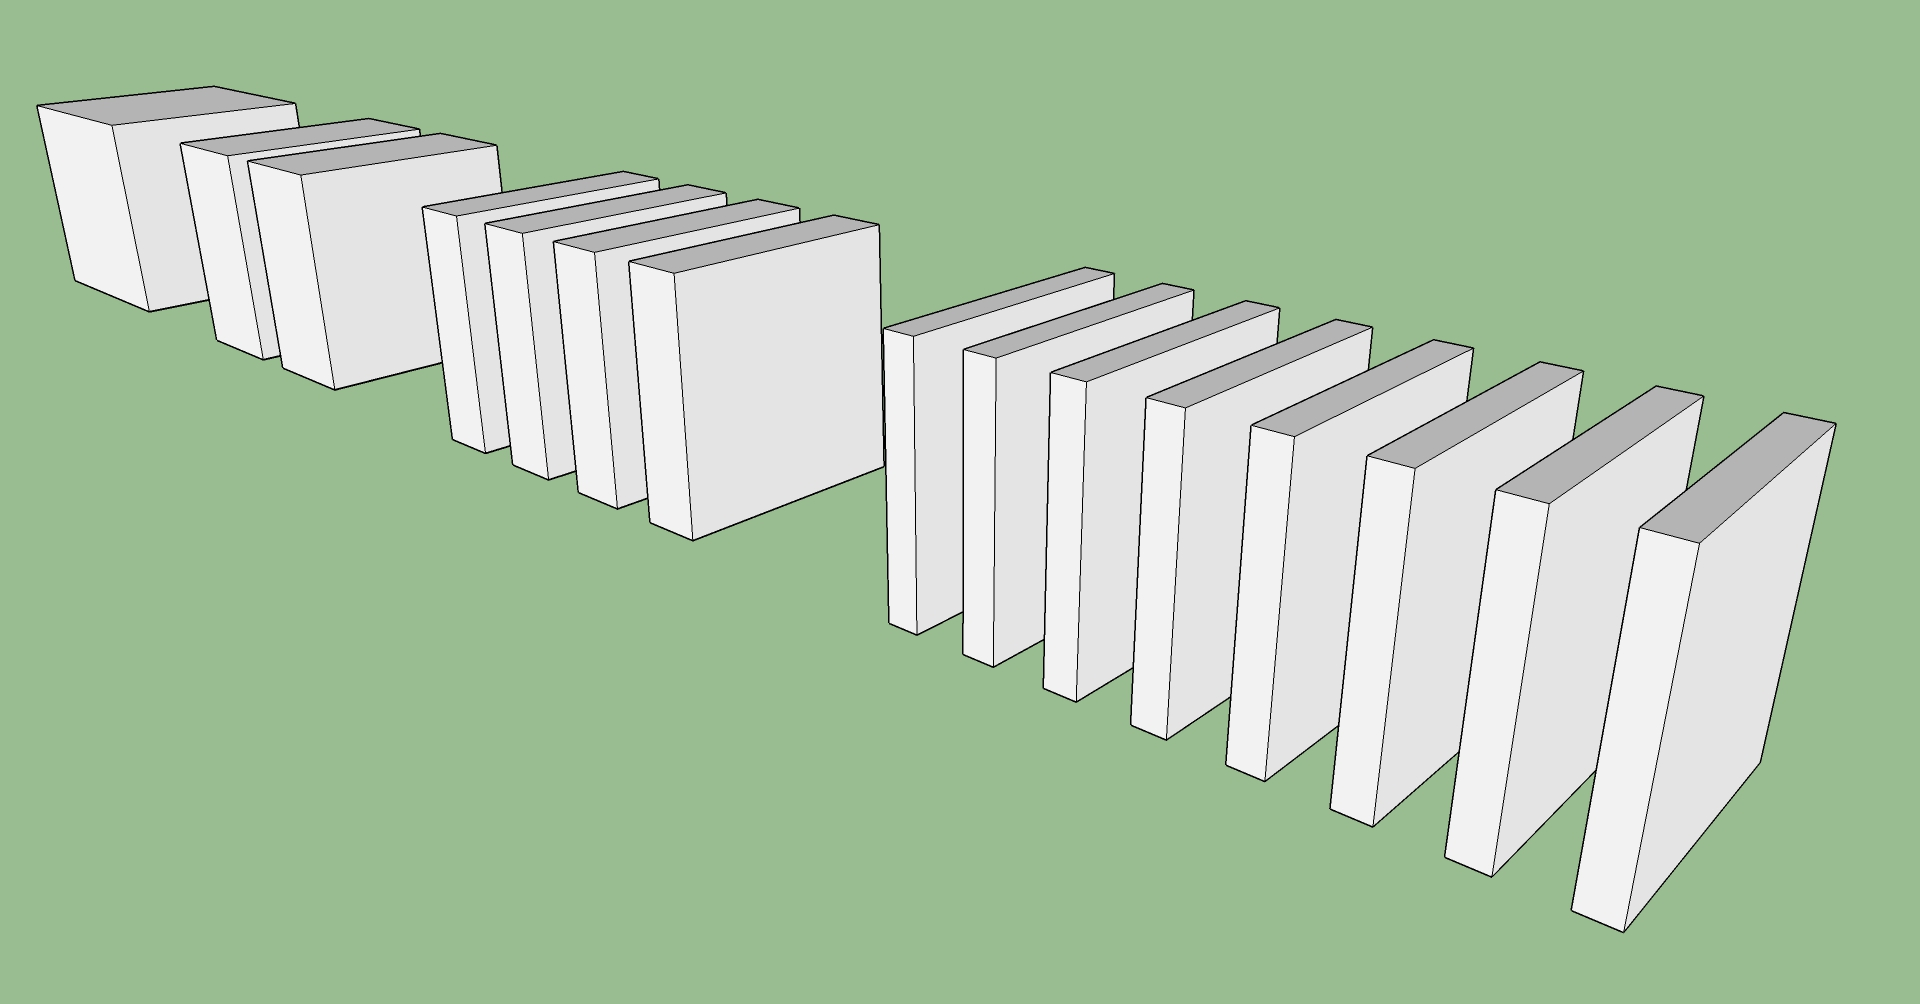
\includegraphics[width=90mm]{cube_division_1.jpg}
		\caption{Particionamiento en la misma dimensión \label{same_dim}}
	\end{figure}

	\begin{figure}[H]
		\centering
		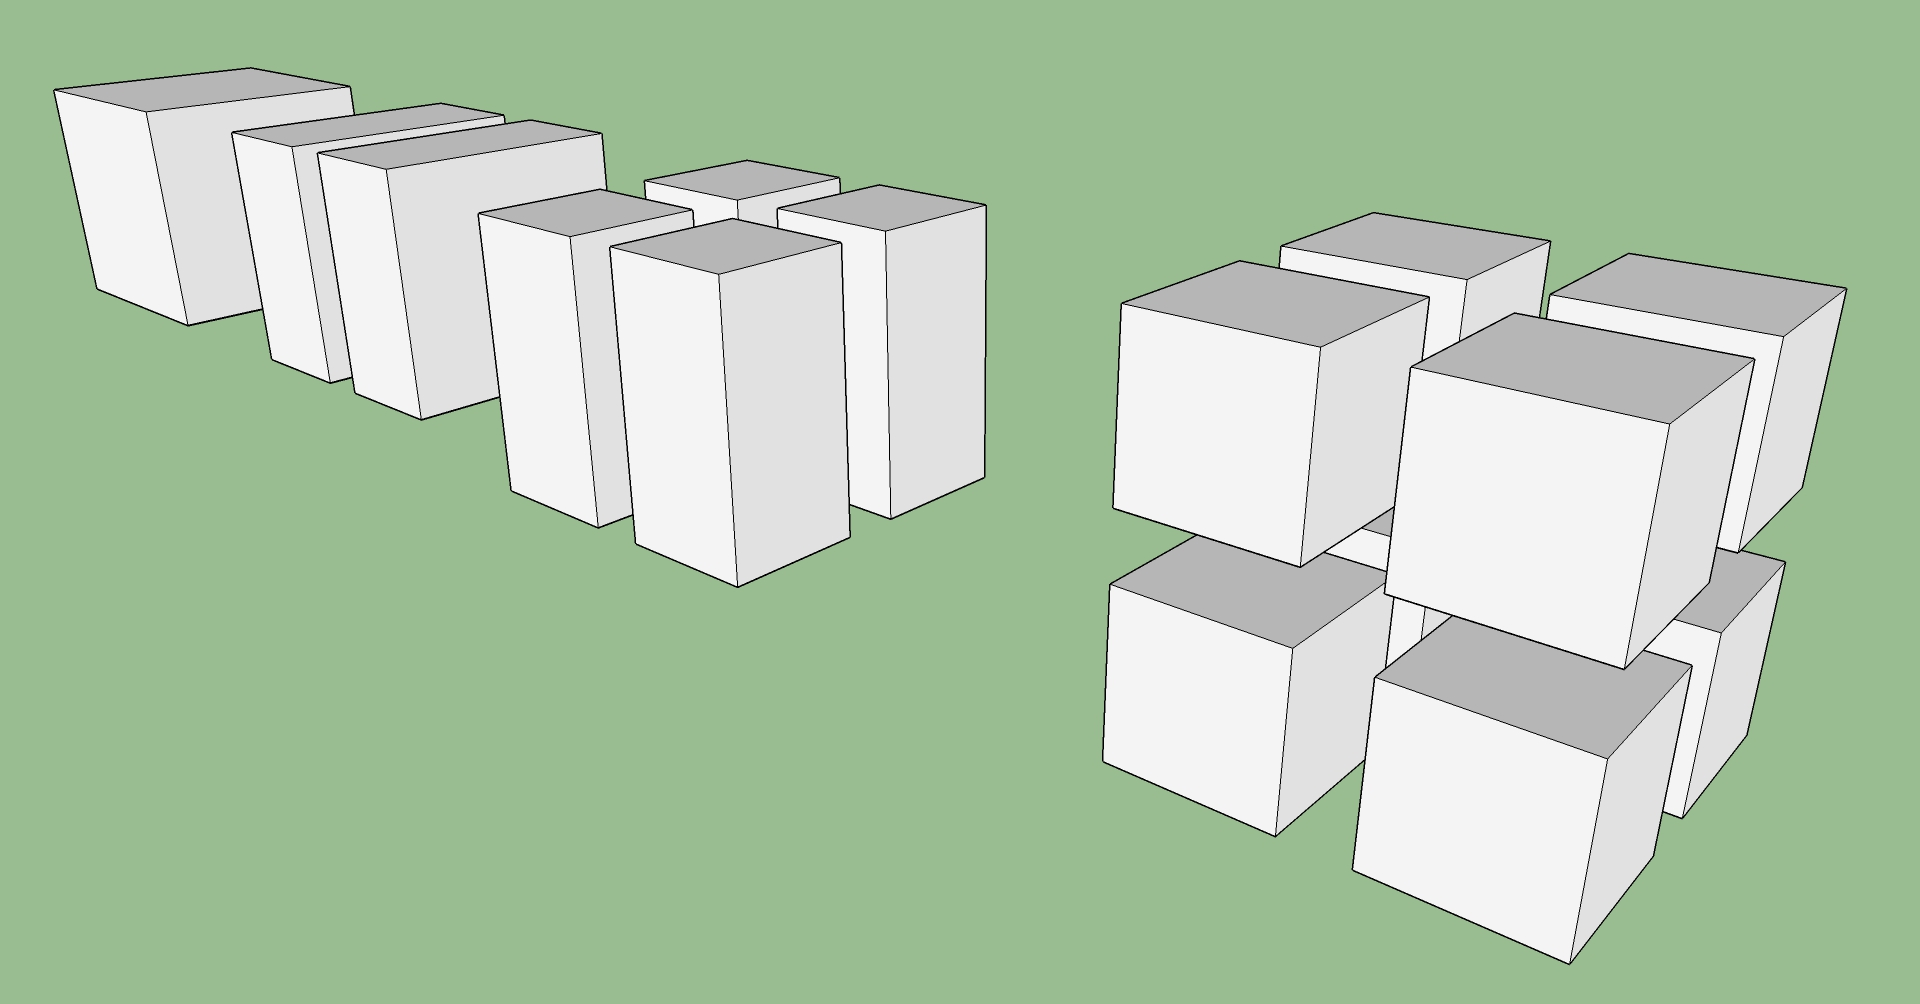
\includegraphics[width=90mm]{cube_division_2.jpg}
		\caption{Particionamiento en distintas dimensiones \label{different_dim}}
	\end{figure}


	\subsection{Combinacion}
		\paragraph{}
		Esta parte corresponde a la combinación de los resultados obtenidos al dividir el subproblema. En lo que se basa es en encontrar cual de los subconjuntos en los que se ha dividido el conjunto de puntos es el que tiene el par con distancia mínima y a la vez evaluar los puntos que están en la frontera entre los subconjuntos, ya que hasta ahora no habíamos tenido en cuenta los pares de puntos que están uno en el primer subconjunto y otro en el segundo subconjunto.
		
		\subsubsection{Encontrar el minimo}

			\paragraph{}
			Esta parte es sencilla, ya que tan solo hay que comparar las distancias de cada par de la partición y quedarse con el que tenga la menor de ellas.

		\subsubsection{Analizar los pares en el punto intermedio}

			\paragraph{}
			Para facilitar el entendimiento del problema lo ilustraremos con la figura \ref{example_border} que corresponde a un ejemplo en 2 dimensiones. Una vez obtenida la distancia minima de los dos subconjuntos en el paso anterior tendremos que estudiar los pares de puntos que cumplen la condición de que uno de ellos esté en el primer subconjunto y otro en el segundo subconjunto.
			
			\paragraph{}
			Ahora deberemos seleccionar el punto más próximo del primer subconjunto respecto del segundo y examinar si la distancia a los puntos del segundo subconjunto es menor que la distancia minima de los dos subconjuntos  que acabamos de calcular en el paso anterior y si es así añadirle al subconjunto de puntos que analizaremos ahora. También habrá que hacer lo mismo pero con los puntos del primer subconjunto (Seleccionar el punto mas próximo del segundo subconjunto respecto del primero y seleccionar los puntos del primero que cumplan la condición antes señalada). Como teníamos los puntos ordenados llegamos a la conclusión de que en cuanto haya un punto que no cumpla la condición todos los siguientes puntos de ese subconjunto ya no la cumplirán, por lo que podemos ahorrarnos también esos cálculos.
			
			\begin{figure}[H]
				\centering
				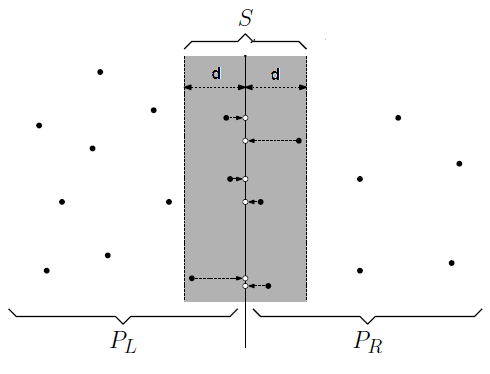
\includegraphics[width=60mm]{strip_closesr1.png}
				\caption{Particionamiento en distintas dimensiones \label{example_border}}
			\end{figure}
			
			\paragraph{}
			Seguidamente, si el subconjunto que acabamos de  definir (el formado por los puntos que están en la frontera de los dos subconjuntos y tienen posibilidad de formar el mínimo) será evaluado aplicando el mismo enfoque se está planteando para solucionar el problema global.

			\paragraph{}
			Una vez obtenido el par con distancia mínima en la zona de la frontera de los dos subconjuntos, es decir, que cumple la condición de que uno de los puntos pertenece a un subconjunto y el otro al otro, se compara con el de los otros otros dos subconjuntos y se selecciona el menor de ellos, que es el mínimo del conjunto.

	\paragraph{}
	Realizando esta operación recursivamente con cada uno de los subconjuntos en los que se va dividiendo el conjunto global en cada nivel de recursión obtendremos el mínimo global de todo el espacio ahorrándonos un gran número de operaciones innecesarias, lo que conlleva una gran mejora de eficiencia.	
	
	\subsection{Pseudocódigo}
		% Insert the algorithm
		\begin{algorithm}[H]

			\caption{Closest Pair algorithm}

			\label{euclid}

			\begin{algorithmic}[1] % The number tells where the line numbering should start

			\Procedure{closestPair}{$P, actDim, dim$} 
				\State $P:$ Conjunto de puntos
				\State $actDim:$ Dimension actual
				\State $dim:$ Número de dimensiones del espacio.
				\State
			
				\If{$len(P) < 3$}
					
					\State \textbf{return}  $bruteForcePair(P)$ 
					\Comment{T(n) = O(1)}
				\Else
					
					\State $actDim\gets(actDim+1) \bmod dim$ 	
					\Comment{T(n) = O(1)}					
					\State $P \gets sort(i, P)$
					\Comment{T(n) = O(nlogn)}
					
					\State
					
					\State $LP \gets P[:len(P)/2]$
					\Comment{T(n) = O(1)}
					
					\State $RP \gets P[len(P)/2:]$
					\Comment{T(n) = O(1)}
					
					\State
					
					\State $LPair \gets closestPair(LP, actDim, dim)$
					\Comment{T(n) = T(n/2)}
					
					\State $RPair \gets closestPair(RP, actDim, dim)$
					\Comment{T(n) = T(n/2)}
					
					\State $LRPair \gets min(LPair, RPair)$
					\Comment{T(n) = O(1)}
					
					\State
					
					\State $MPair \gets closestMidle(LRPair, LP, RP, actDim, dim)$
					\Comment{T(n) = U(n)}
					
					\State

					\State \textbf{return} $min(MPair, LRPair)$
					\Comment{T(n) = O(1)}
	
				\EndIf
			
			\EndProcedure

			\end{algorithmic}

		\end{algorithm}
		
		
		\begin{algorithm}[H]

			\caption{closestMidle}

			\label{closestMidle}

			\begin{algorithmic}[1] % The number tells where the line numbering should start

			\Procedure{closestMidle}{$LRPair, LP, RP, actDim, dim$} 
				\State $LRPair:$ Par mínimo encontrado de los dos subconjuntos
				\State $LP:$ Primer subconjunto de puntos
				\State $RP:$ Segundo subconjunto de puntos
				\State $actDim:$ Dimension actual
				\State $dim:$ Número de dimensiones del espacio.
				\State

			
				\State $d \gets LRPair.distance()$
				\Comment{T(n) = O(1)}

				\State $LBorderPoint \gets RP[0]$
				\Comment{T(n) = O(1)}

				\State $RBorderPoint \gets LP[-1]$
				\Comment{T(n) = O(1)}

				\State
				
				\State $MP \gets points: d > \abs{LBorderPoint[actDim] - point[actDim]} \in RP$
				\Comment{T(n) = O(n)}

				\State $MP \gets MP \cup points:  d > \abs{RBorderPoint[actDim] - point[actDim]} \in LP$
				\Comment{T(n) = O(n)}

				\State	
								
				\State \textbf{return} $closestPair(MP, actDim, dim)$
				\Comment{T(n) = T(n/k)}


			\EndProcedure

			\end{algorithmic}

		\end{algorithm}

	\subsection{Análisis de crecimiento}
	
		\paragraph{}
		Las ecuaciones de recurrencia de la primera función y segunda funciones respectivamente son:
	
		\begin{equation}
		T(n) =  2T(n/2) + U(n) + O(nlogn)
		\end{equation}
		
		\begin{equation}
		U(n) = T(n/k) + 2O(n)
		\end{equation}

		\paragraph{}
		La variable $k$ hace referencia a la cantidad de puntos que se han descartado del análisis por estar mas alejados de un punto del otro subconjunto que la distancia del mñinimo par encontrado en los subconjuntos. Esta variable toma valores en el intervalo $(1, +\infty)$ tendiendo a $+\infty$ si estamos estudiando un espacio de dimensiones pequeñas y tendiendo a valores cercanos a 1 si nuestra espacio tiene una dimensión muy grande. Aplicando el teorema maestro sobre la primera y la segunda ecuaciones de recurrencia obtenemos:
		
		\begin{equation}
			U(n) = O(logn)
		\end{equation}
		
		\begin{equation}
			T(n) = 2T(n/2) +  O(logn) + O(nlogn) = 2T(n/2) + O(nlogn) = O(nlogn)
		\end{equation}
		
		Pero este resultado no está del todo ajustado, ya que en los cálculos no apararece la dimensión, que como hemos dicho influye en el crecimiento asintótico. Gracias a la información obtenida a partir de la bibliografía (concretamente al segundo enlace que aparece en el listado de referencia bibliográfica.) se llega a la conclusión de que $O(nlogn^{d-1})$ es una mejor aproximación.
		
	\subsection{Desventajas de esta solución}
	

		\paragraph{}
		Con esta estrategia conseguimos concentrar los puntos en subconjuntos respecto de un eje de coordenadas cada vez, lo que nos proporciona cercanía "real" entre los puntos de cada subconjunto en el caso de trabajar con dimensiones pequeñas.
		
		\paragraph{}
		La causa de esto se debe a que el valor de la posición se "concentra" en pocos valores (3 en el caso de 3 dimensiones) por lo que podemos acotar mejor la situación del punto fijándonos en uno de ellos. Burdamente hablando controlamos $1/3$ del punto. Mientras que si estamos estudiando puntos de dimensión 100 en cuyo caso tendriamos 100 valores por cada punto burdamente hablando tan solo controlamos la posición del punto en $1/100$
		
		\paragraph{}
		El cuello de botella de esta solución se encuentra en la fase de selección de los puntos que se encuentran en la frontera entre los dos subconjuntos en los que se divide el problema y se acentúa gravemente cuando la dimension del espacio toma valores elevados.
		
		\paragraph{Aclaración:}
		La solución implementada y aquí explicada no es la óptima para dimensiones superiores a 2, ya que esta tiene un crecimiento asintótico de $O(nlogn^{d-1})$ donde $d = $ dimension del espacio. La solución expuesta en el apartado siguiente tiene un mejor crecimiento asintótico.
		
\section{Solución Óptima}
	\paragraph{}
	La solución óptima al problema de encontrar el par de puntos más cercano en un espacio n-dimensional se puede conseguir con un crecimiento asintótico de $O(nlogn)$, es decir, sin que dependa la dimensión en el crecimiento. Esto se consigue mediante la utilización de hiperplanos, que nos dan la ventaja de poder reducir la dimensión del espacio. Con este método se llega a la siguiente ecuación de recurrencia:
	$T(n, d) = 2T(n/2, d) + U(m, d - 1) + O(n)$ donde $U(m, d-1)=O(m (logm) d - 2) = O(n)$. Simplificando llegamos a $T(n,d)=2T(n/2,d)+O(n)+O(n)$ que se resuelve en $O(nlogn)$ 

\section{Referencia Bibliográfica}

	\begin{itemize}
		\item \url{https://es.wikipedia.org/wiki/Algoritmo_divide_y_venceras}	
		
		\item \url{https://www.cs.ucsb.edu/~suri/cs235/ClosestPair.pdf}	
		
		\item \url{https://en.wikipedia.org/wiki/Closest_pair_of_points_problem}
		
		\item \url{https://people.csail.mit.edu/indyk/ohad.ps}
		
		\item \url{http://www.geeksforgeeks.org/closest-pair-of-points/}	
		
		\item \url{https://people.csail.mit.edu/indyk/6.838-old/handouts/lec17.pdf}	
		
		\item \url{https://courses.cs.washington.edu/courses/cse421/11su/slides/05dc.pdf}
		
	\end{itemize}


\end{document}
